%%%%%%%%%%%%%%%%%%%%%%%%%%%%%%%%%%%%%%%%%%%%%%%%%%%%%%%%%%%%%%%%%%%%%%%%%%%%%%%%
%2345678901234567890123456789012345678901234567890123456789012345678901234567890
%        1         2         3         4         5         6         7         8
\documentclass[letterpaper, 10 pt, conference]{ieeeconf}  % Comment this line out
                                                          % if you need a4paper
%\documentclass[a4paper, 10pt, conference]{ieeeconf}      % Use this line for a4

\usepackage{float}
                                                          % paper
% uso paquete bookmark para tener bien los outlines.
\usepackage{bookmark}

% Configuro el idioma.
\usepackage[utf8]{inputenc} % Importante para mantener acentos.
\usepackage[spanish, activeacute]{babel} % Requiere: texlive-lang-spanish. Por primera vez hay que ejecutar: texconfig init> log

% Paquete para poder usar acentos en $$.
\usepackage{mathtools}
%\setmathfont{XITS math}

% Para los diagramas de flujo
\usepackage{tikz}
\usetikzlibrary{shapes.geometric, arrows}

% Elementos del diagrama
\tikzstyle{startstop} = [rectangle, rounded corners, 
minimum width=6em, 
minimum height=2em,
text centered, 
draw=black, 
fill=red!30]

\tikzstyle{io} = [trapezium, 
trapezium stretches=true, % A later addition
trapezium left angle=70, 
trapezium right angle=110, 
minimum width=6em, 
minimum height=2em, text centered, 
draw=black, fill=blue!30]

\tikzstyle{block} = [rectangle, 
minimum width=8em, 
minimum height=3em, 
text centered, 
text width=7.5em, 
draw=black, 
fill=white!30]

\tikzstyle{def} = [rectangle, 
minimum width=14em, 
minimum height=3em, 
text centered, 
text width=12em, 
draw=black, 
fill=purple!30]

\tikzstyle{swap_proccess} = [rectangle, 
minimum width=8em, 
minimum height=2em, 
text centered, 
text width=8em, 
draw=black, 
fill=orange!30]

\tikzstyle{process} = [rectangle, 
minimum width=6em, 
minimum height=2em, 
text centered, 
text width=6em, 
draw=black, 
fill=orange!30]

\tikzstyle{decision} = [diamond, 
minimum width=6em, 
minimum height=6em, 
text centered, 
draw=black, 
fill=green!30]
\tikzstyle{arrow} = [thick,->,>=stealth]

\usepackage{siunitx}

% package to get \url
\usepackage{hyperref}
\hypersetup{
  colorlinks=true,
  linkcolor=magenta,
  filecolor=magenta,
  citecolor=magenta,      
  urlcolor=magenta,
}

% Graficos electrónicos
\usepackage{circuitikz}

\IEEEoverridecommandlockouts                              % This command is only
                                                          % needed if you want to
                                                          % use the \thanks command
\overrideIEEEmargins
% See the \addtolength command later in the file to balance the column lengths
% on the last page of the document

\usepackage{graphicx}
\usepackage{graphics}

% styling for matlab/octave code.
\usepackage{matlab-prettifier}
% Configuracion, con esto puede agregar ñ.
\lstset{
  literate={ñ}{{\~n}}1
}

\usepackage{listings}

% The following packages can be found on http:\\www.ctan.org
%\usepackage{graphics} % for pdf, bitmapped graphics files
%\usepackage{epsfig} % for postscript graphics files
%\usepackage{mathptmx} % assumes new font selection scheme installed
%\usepackage{times} % assumes new font selection scheme installed
\usepackage{amsmath} % assumes amsmath package installed
%\usepackage{amssymb}  % assumes amsmath package installed

\title{\LARGE \bf Laboratorio N° 1}

\author{
  Tom\'as Vidal\\
  {\it Control Automático II}\\
  {\it Facultad de Ingenier\'ia, UNLP, La Plata, Argentina.}\\
  {\it 6 de Mayo, 2024.}
}                                            % <-this % stops a space


% comienzo

% INTRO


% Figura
\newcommand{\image}[2] {
  \begin{figure}[H]
    \centering
    \includegraphics[width=0.43\textwidth]{./#1.png}
    \caption{#2}
    \label{fig:#1}
  \end{figure}
}

% Codigo
% \begin{lstlisting}[style=Matlab-editor]
% % el código va aca
% dispc("HELLO WORLD");
% \end{lstlisting}

\begin{document}
\maketitle
\thispagestyle{empty}
\pagestyle{empty}

\section{Diagrama Eléctrico Esquemático}
\begin{figure}[H]
  \centering
  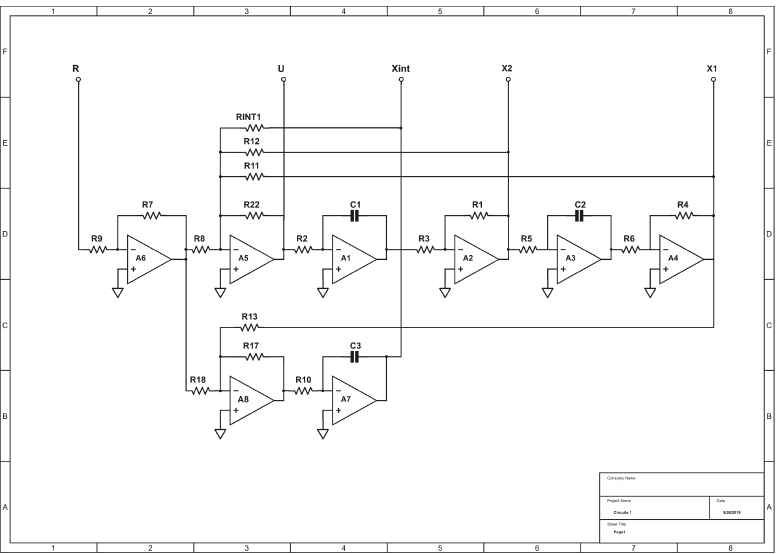
\includegraphics[width=0.43\textwidth]{./Imagenes/DiagElecEsquematico.png}
  \caption{Diagrama eléctrico esquemático del circuito provisto}
  \label{fig:diag_elect_esq}
\end{figure}

En el diagrama \ref{fig:diag_elect_esq} se pueden identificar diferentes bloques que cumplen distintas funciones. Estos están identificados en el diagrama \ref{fig:diag_elec_esq_etapas}, y sus funciones se detallan a continuación:
\begin{itemize}
  \item \textbf{Inversor:} crea un desfase de \ang{180} a la salida respecto de la entrada (\textit{color rojo}).
  \item \textbf{Sumador inversor:} suma todas las señales en la entrada y luego desfasa el resultado en \ang{180} (\textit{color azul}).
  \item \textbf{Integrador inversor:} integra la señal de entrada y la desfasa en \ang{180}  (\textit{color verde}).
\end{itemize}
\begin{figure}[H]
  \centering
  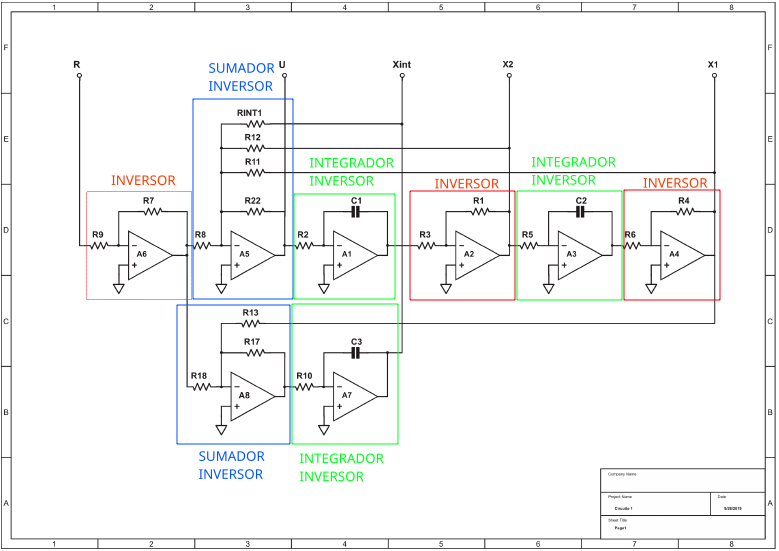
\includegraphics[width=0.43\textwidth]{./Imagenes/DiagElecEsqEtapasIdent.png}
  \caption{Se identifican las etapas funcionales del diagrama \ref{fig:diag_elect_esq}}
  \label{fig:diag_elec_esq_etapas}
\end{figure}

%\subsection{Lógica del programa}
%La implmentación del algoritmo de la figura \ref{diag:flujo} en sí se realizó en la subrutina de la figura \ref{code:bubble_sort}, el resto del código se enfoca en cargar los datos de prueba y adecuar las posiciones de memoria especificadas correctamente. La extensión del código se debe a su \textit{alta organización}, \textit{documentación} y \textit{buenas prácticas generales}, porque de otra manera el algoritmo por sí solo no hubiera llevado tantas líneas. El siguiente diagrama explica mejor el flujo general del programa.
%\begin{figure}[H]
%  \tiny
%  \centering
%  \label{diag:bloques_gen}
%  \begin{tikzpicture}[node distance=2cm]
%
%  \node (start) [block] {Comienzo};
%  \node (ic1) [block, right of=start] {Cargar condiciones iniciales};
%  \node (test_data) [block, right of=ic1] {Cargar vector de prueba y su longitud};
%  \node (ic2) [block, right of=test_data] {Cargar condiciones iniciales};
%  \node (print1) [block, below of=ic2] {Mostrar vector en la salida};
%  \node (sort) [block, left of=print1] {Ordenar el vector de menor a mayor};
%  \node (print2) [block, left of=sort] {Mostrar vector en la salida};
%  \node (end) [block, left of=print2] {Fin};
%
%  \draw [arrow] (start) -- (ic1);
%  \draw [arrow] (ic1) -- (test_data);
%  \draw [arrow] (test_data) -- (ic2);
%  \draw [arrow] (ic2) -- (print1);
%  \draw [arrow] (print1) -- (sort);
%  \draw [arrow] (sort) -- (print2);
%  \draw [arrow] (print2) -- (end);
%
%\end{tikzpicture}
%\end{figure}
%Como se puede observar se cargan dos veces las condiciones iniciales (es una forma de decirle a los valores que toman las variables inicialmente), esto se debe a que el primer \textit{seteo} es por si se quiere reiniciar el programa sin tener que reensamblar el código, y la segunda condición es debido a que al principio se cargan los datos del vector de prueba en la posición de memoria correcta, y para esto se reutilizan variables empleadas posteriormente en el algoritmo de organización del vector de datos, por lo que se requiere un reestablecimiento de los valores inciales de las mismas.
%
%\subsection{Algoritmo implementado}
%El algoritmo de Bubble Sort implementado se hizo a partir del diagrama de flujo \ref{diag:flujo}, en el código de se puede apreciar que se documenta cada parte acorde a este diagrama. De todas formas se hará una breve explicación del mismo. La subrutina consiste básicamente en dos bucles (\textit{iIndex} y \textit{jIndex}) que basados en ciertas condiciones hacen cambiar el dato contenido en la posición de memoria: \textbf{0x0002 + j}, es decir $a[j]$, con el valor de $a[j+1]$. La condición justamente sería que si $a[j]$ es mayor que $a[j+1]$ (el valor anterior es mayor que el posterior) hay que hacer la permutación de los datos, para lo cual se debe almacenar temporalmente uno de los datos mientras se hace dicha permutación (en el código: \textit{aJAddr} y \textit{aJData}), una vez que se concreta el recorrido del bucle de \textit{iIndex} (que es el que contiene a \textit{jIndex}) se da por finalizada la organización del vector y se sale de esta subrutina. También cabe aclarar que esta subrutina tiene al comienzo una sección en la que se indican condiciones inciales.
%\begin{figure}[H]
%  \footnotesize
%  % \centering
%  \begin{tikzpicture}[node distance=1.1cm]
%
%    \node (start) [startstop] {Comienzo};
%    \node (initcond) [def, below of=start] {a = $<a_0, a_1, \dots, a_n>$};
%    \node (def_i_j) [def, below of=initcond] {i=0; j=0};
%
%    \node (i_less_n) [decision, below of=def_i_j, yshift=-0.5cm] {$i<n$};
%    \node (print_arr) [process, right of=i_less_n, xshift=2.75cm] {Imprimir arreglo};
%    \node (end) [startstop, below of=print_arr, yshift=-0.25cm] {Terminar};
%
%    \node (j_less_n) [decision, below of=i_less_n, yshift=-1.5cm] {$j<n-i-1$};
%    \node (inc_i) [process, left of=j_less_n, xshift=-1.4cm, yshift=1.75cm] {$i = i+1$};
%
%    \node (a_gtr_a1) [decision, below of=j_less_n, yshift=-1.75cm] {$a[j]>a[j+1]$};
%    \node (inc_j) [process, right of=a_gtr_a1, xshift=1.5cm] {$j = j+1$};
%
%    \node (swap) [swap_proccess, below of=a_gtr_a1, yshift=-1cm] {permutar $ a[j] \leftrightarrow a[j+1]$};
%
%    \draw [arrow] (start) -- (initcond);
%    \draw [arrow] (initcond) -- (def_i_j);
%    \draw [arrow] (def_i_j) -- (i_less_n);
%    \draw [arrow] (i_less_n) -- node[anchor=south] {no} (print_arr);
%    \draw [arrow] (print_arr) -- (end);
%    \draw [arrow] (i_less_n) -- node[anchor=west] {si} (j_less_n);
%    \draw [arrow] (j_less_n) -| node[anchor=south, xshift=1cm] {no} (inc_i);
%    \draw [arrow] (j_less_n) -- node[anchor=west] {si} (a_gtr_a1);
%    \draw [arrow] (inc_i.north) |- (i_less_n.west);
%    \draw [arrow] (a_gtr_a1) -- node[anchor=west] {si} (swap);
%    \draw [arrow] (a_gtr_a1) -- node[anchor=south] {no} (inc_j);
%    \draw [arrow] (swap) -| (inc_j);
%    \draw [arrow] (inc_j.north) |- (j_less_n.north);
%
%  \end{tikzpicture}
%  \caption{Diagrama de flujo de Bubble Sort}
%  \label{diag:flujo}
%\end{figure}
%
%\begin{figure}
%  \lstinputlisting[breaklines=false, firstline=45, lastline=129, frame=L, basicstyle=\tiny, caption={Fragmento del código \textit{``69854\_1\_0.asm''}}, label={code:bubbleSort}]{../programas_tp_1/69854_1_0.asm}
%  \caption{Segmento del código que contiene la subrutina de ordenamiento}
%  \label{code:bubble_sort}
%\end{figure}
%
%\subsection{Memoria ocupada}
%Para poder funcionar, el programa ocupa 122 instrucciones en total, contenidas en las direcciones \textbf{0x0100} hasta \textbf{0x0179} (en hexadecimal); de las cuales 9 son empleadas para variables (memoria de datos).
%
%\section{Resultados de instrucciones}
%Para analizar el rendimiento o eficacia del programa una metrica que se puede emplear es la cantidad de instrucciones que le lleva al programa efectuar la organización de los datos, y esta misma es la forma en que se midió el rendimiento. Como se explicó previamente en la sección \ref{sec:bubble_sort} se espera que la cantidad de instrucciones para cada vector sea aproximadamente la misma, independientemente de los datos de los vectores \textit{(suponiendo vectores de mismas dimensiones)}, aunque primero se analizará como son los resultados relativos. Imaginemos que tenemos un vector ya \textbf{ordenado}, entonces nunca se entraría en el bucle de permutar los datos, por lo cual este sería el caso con menos instrucciones. Ahora si imaginamos un vector con todos los datos desordenados (vector \textbf{invertido}), es decir que habría que permutarlos a todos, en este caso se ejecutarían la máxima cantidad de instrucciones, por lo que sería el caso con más instrucciones. Y por último (caso más típico) si tenemos un vector con sólo algunos datos ordenados (vector \textbf{desordenado}), llevaría más instrucciones que el primer caso, pero menos que el segundo. Y esto mismo ocurrió en el resultado de la tabla \ref{tab:instrucciones}.
%
%\begin{table}[H]
%  \centering
%  \begin{tabular}{|l|l|l|l|}
%    \hline
%                  & Ordenado & Desordenado & Invertido \\ \hline
%    Solo ordenamiento & 534      & 567         & 597       \\ \hline
%    Programa entero   & 853      & 886         & 916       \\ \hline
%  \end{tabular}
%  \caption{Instrucciones para organizar cada vector}
%  \label{tab:instrucciones}
%\end{table}
%
%Los vectores empleados para realizar la tabla \ref{tab:instrucciones} son los siguientes:
%
%\begin{table}[H]
%  \centering
%  \begin{tabular}{|l|l|l|}
%    \hline
%    Ordenado                                & Desordenado                             & Invertido                               \\ \hline
%    \textless-3,-2,-1,0,1,2,3\textgreater   & \textless0,-2,1,3,-1,2,-3\textgreater   & \textless3,2,1,0,-1,-2,-3\textgreater   \\ \hline
%  \end{tabular}
%  \caption{Vectores empleados para en análisis}
%  \label{tab:vectores}
%\end{table}
%
%\section{Conclusiones}
%Se concluye que el algoritmo funciona como se esperaba, y que la ventaja del mismo es que no depende tanto de los datos, sino que lo hace más de su dimensión. Además se debe tener en cuenta que si bien la dimensión de los vectores es $7$ y que las instrucciones medidas fueron de media $566$ (es decir que uno esperaría que fueran $7^{2}$) no significa que esté mal, sino que es el conjunto de instrucciones que permutan los datos, los que son ejecutados $49$ veces, y que en la arquitectura MARIE se está limitado a hacer ciertas tareas básicas, como alojar datos en una variable o redirijir el flujo del programa, con varias instrucciones, por esto mismo es que le lleva tantos ciclos de reloj a la arquitectura completar la tarea.

\end{document}
